

\section{Evaluation Metrics}
\label{appendix:human_rate}
We use the automatic metric ROUGE-L~\cite{lin2002manual} to assess the quality of the generated text by comparing it with reference answers. In addition, we incorporate manual checking into the evaluation pipeline and compute a human-rating score. Five evaluators with biological-research experience were asked to rate each generated answer on a 0–5 scale (the integer score corresponds to the category number minus one). All evaluators have at least two years of research experience in biology. The six ordinal categories they used are:

\begin{enumerate}
  \item \textbf{Garbled} -- the text is incomprehensible and lacks any readability.
  \item \textbf{Inaccurate} -- the text is readable but entirely incorrect and devoid of meaningful information.
  \item \textbf{Partially informative} -- the text offers some reference value, yet its factual correctness is poor.
  \item \textbf{Moderately accurate} -- roughly half of the information is correct, but several errors remain.
  \item \textbf{Mostly accurate} -- the content is almost entirely correct, with only minor omissions or errors.
  \item \textbf{Completely correct} -- the content is accurate in its entirety, without any mistakes.
\end{enumerate}

\section{ADDITIONAL RESULTS}

\paragraph{Evaluation on real-world protein scenarios} 
To examine the applicability of our framework beyond benchmark datasets, we evaluated it on biologically relevant queries involving uncharacterized \textit{Homo sapiens} proteins. For each case, a current biologically relevant question of research interest was paired with the corresponding protein amino acid sequence and input to representative LLMs guided by our framework. As illustrated in Figure~\ref{fig:realworld_study}, the models produced plausible hypotheses aligned with biological knowledge. These results demonstrate that our framework can extend to real-world scenarios, offering interpretable preliminary insights into proteins lacking experimental annotation and potentially guiding future biological investigations.
\begin{figure}[ht]
\centering
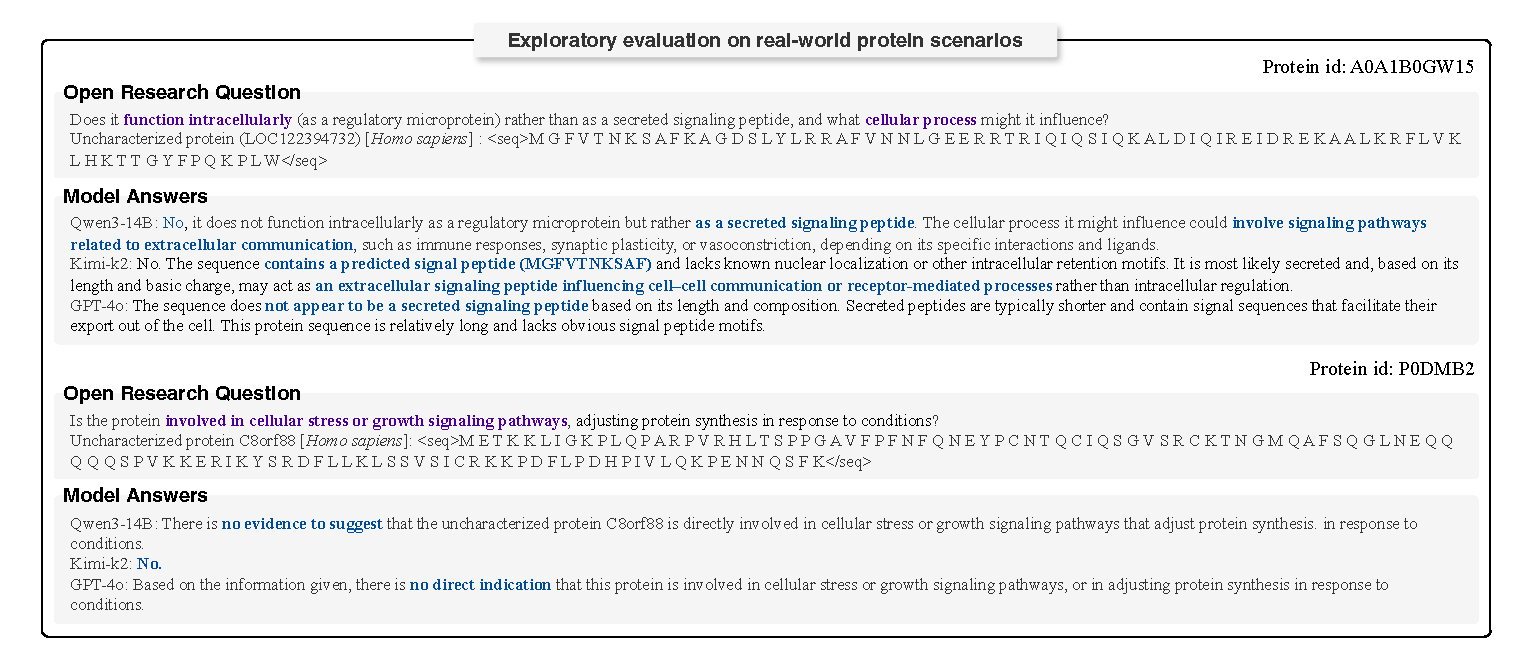
\includegraphics[width=\linewidth]{figure/realworld.pdf}
\caption{\textbf{Exploratory evaluation of our framework on real-world protein scenarios.}  
}
\label{fig:realworld_study}
\end{figure}

\section{Bilingual Dataset: Details and Examples}
\label{appendix:dataset_detail}

All protein entries are derived from the manually curated SwissProt~\cite{bairoch2000swiss} section of UniProt, which provides high-quality annotations of protein sequences and functional descriptions. After deduplication, we prompted LLMs to generate four types of bilingual QA pairs from these entries. To assess data quality, we randomly sampled 500 pairs from the full set of 79,926 automatically constructed examples. Each sampled pair was manually reviewed by domain experts along three dimensions: semantic fidelity, biological plausibility, and translation fluency. The review showed a 95\% pass rate, confirming that the dataset maintains high linguistic accuracy and biological reliability. Examples of four bilingual QA types are provided in Figure~\ref{fig:dataset_example_p1} and Figure~\ref{fig:dataset_example_p2}.
\begin{figure}[htbp]
  \centering
  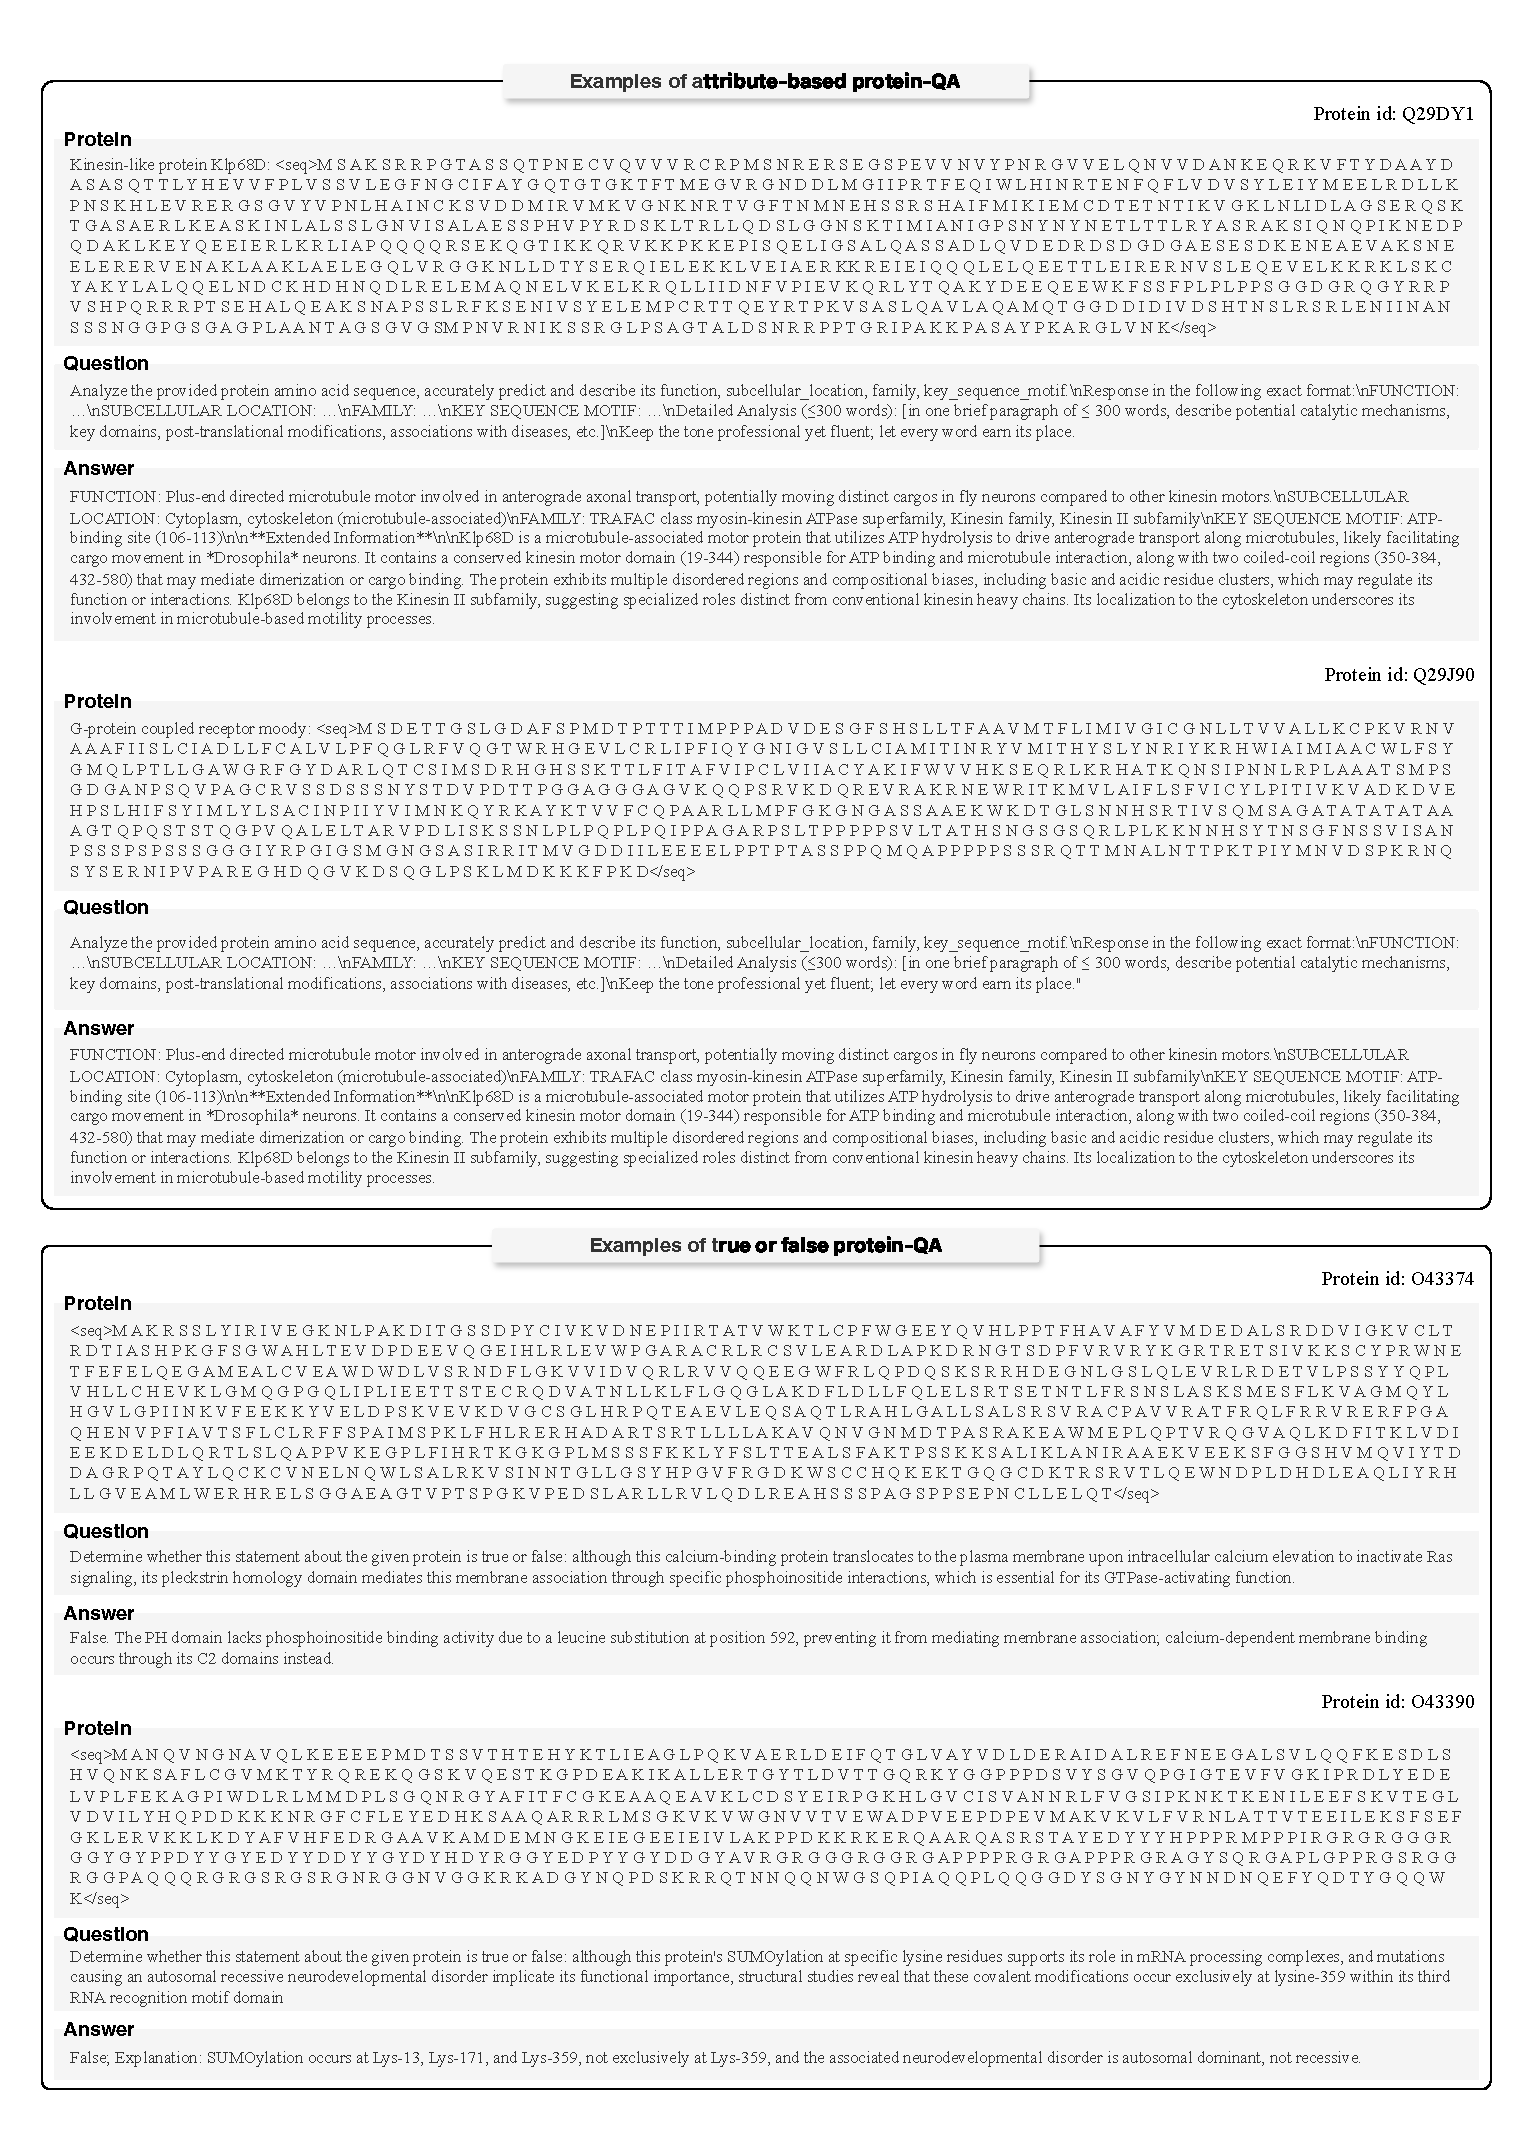
\includegraphics[width=\linewidth]{figure/dataset_example_p1.pdf}
  \caption{\textbf{Illustrative examples of the four bilingual QA types (Part 1).}}
  \label{fig:dataset_example_p1}
\end{figure}

\begin{figure}[htbp]
  \centering
  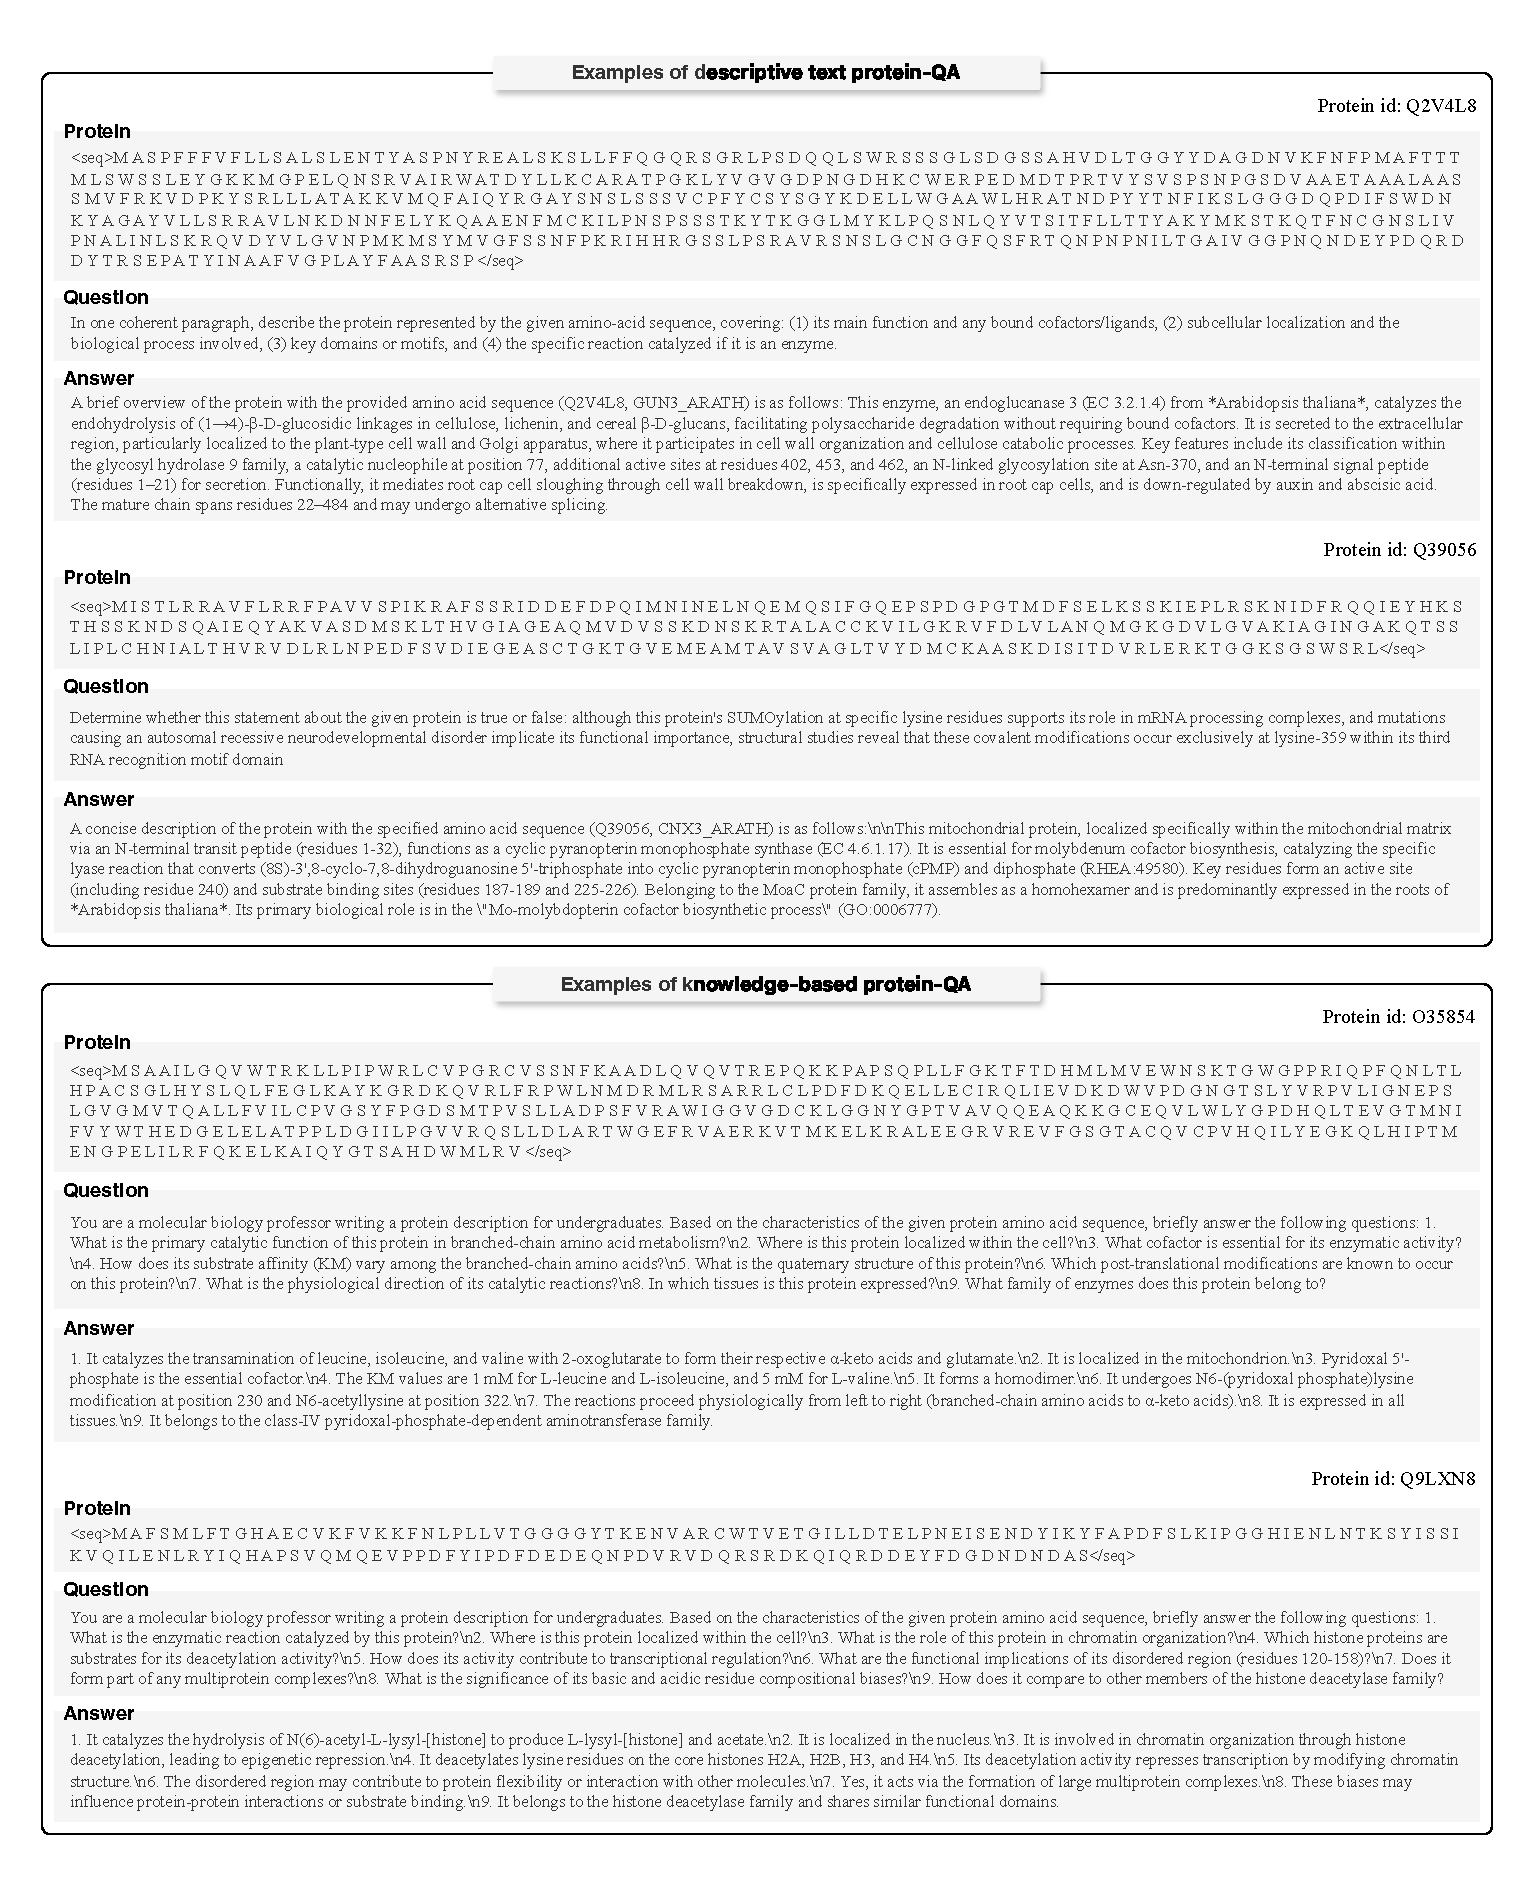
\includegraphics[width=\linewidth]{figure/dataset_example_p2.pdf}
  \caption{\textbf{Illustrative examples of the four bilingual QA types (Part 2).}}
  \label{fig:dataset_example_p2}
\end{figure}

\section{llm statement}
\label{appendix:llm_prompt}
We acknowledge the use of LLMs in this work. Specifically, DeepSeek-R1~\cite{guo2025deepseek} was employed for two purposes: (i) polishing the English presentation of the manuscript, and (ii) generating bilingual dataset entries from curated protein annotations, where the prompts were carefully designed to ensure scientific accuracy and linguistic quality. Below we provide the exact prompts used for each bilingual QA type in the dataset construction process. 

Prompt for \texttt{Attribute-based Answer} generation is following:
\begin{scriptsize}\begin{verbatim}
"Based on the provided annotations, compose a concise protein information description in the 
following fixed format: 
PROTEIN NAME: …
FUNCTION: …
SUBCELLULAR LOCATION: …
FAMILY: …
KEY SEQUENCE MOTIF: … (write N/A if none).
After the fixed fields, leave one blank line and proceed to the `Extended Information' 
paragraph. In fluent, professional English, supply any additional details essential for 
understanding the protein, integrating all relevant annotation content in a coherent 
narrative. Maintain brevity and avoid redundancy."
\end{verbatim}\end{scriptsize}

Prompt for \texttt{True or False QA} generation is following:
\begin{scriptsize}\begin{verbatim}
"You are a protein science expert. Please read the UniProt entry above and design 1 True/False 
question that meets all of the following rules: 
(1) The stem must weave together diverse distinct knowledge dimensions from the entry (e.g.,
catalytic chemistry, structural biology, disease relevance, evolutionary conservation, PTM,
mutational effect, regulatory mechanism, substrate selectivity, experimental evidence, 
GO term, PDB ID, cofactor, physiological pathway, drug-target potential). 
(2) Do not include the words `True/False' in the stem; hide the decisive technical point 
within the details. 
(3) Give True or False, followed by an explanation. 
Use this exact output template: Stem: …; Answer: …; Explanation: …"
\end{verbatim}\end{scriptsize}

Prompt for \texttt{Descriptive Text} generation is following:
\begin{scriptsize}\begin{verbatim}
"Based on the given annotation information of the protein, describe the given amino-acid 
sequence in one coherent paragraph that covers: 
(1) its main function and any bound cofactors/ligands, 
(2) subcellular localization and the biological process involved, 
(3) key domains or motifs, and 
(4) the specific reaction catalyzed if it is an enzyme. The description begins with A 
sentence pattern like 
`A short report on the protein with the given amino acid sequence highlights:'
or `A brief overview of the protein with the provided amino acid sequence is as follows:' 
or `A concise description of the protein with the specified amino acid sequence includes:'
or `An outline of the key aspects of the protein with the corresponding amino acid sequence 
is as follows:' 
or `A summary of the protein's main attributes with the input amino acid sequence reveals:' 
(uses similar synonymous sentences to avoid uniformity)."
\end{verbatim}\end{scriptsize}

Prompt for \texttt{Knowledge-based QA} generation is following:
\begin{scriptsize}\begin{verbatim}
"Based on the provided annotations, generate exactly 1-9 distinct, single-sentence questions 
that a researcher would naturally ask to fully interrogate this protein. Guidelines:
(1) Each question must probe a different biological dimension (expression, localization, 
mechanism, regulation, phenotype, disease, evolution, interaction, structure/properties).
(2) Keep questions concise, fluent.
(3) One per line, numbering, and the corresponding answers to these questions are concise and 
clear.
(4) The questions can be appropriately flexible and occasionally combined with some actual 
scenarios or content related to species.
The Questions and Answers are divided into two parts (wrapped with <Questions><\\Questions> 
and <Answers><\\Answers> respectively). All the information in the Q&A should be based entirely 
on the given annotations and should not be supplemented by yourself."
\end{verbatim}\end{scriptsize}


